% !TeX program = xelatex
\documentclass[a4paper, 12pt]{article}

\usepackage[brazil]{babel}
\let\latinencoding\relax
\usepackage[T1]{fontenc}

\usepackage[no-math]{fontspec}
\usepackage{newpxtext, newpxmath}
\usepackage[a4paper, margin=2cm]{geometry}
\usepackage{pdflscape}
\usepackage{graphicx}
\usepackage{float}
\usepackage{rotating}
\usepackage{pdflscape}
\PassOptionsToPackage{hyphens}{url}
\usepackage[colorlinks,urlcolor=blue,linkcolor=black]{hyperref}
\usepackage{siunitx}
\usepackage[os=win]{menukeys}
\usepackage{minted}
\usepackage{booktabs}
\usepackage{array}
\usepackage{xcolor}

\input{definition.tex}

\title{\titulo}
\author{\nomeAutorUm e \nomeAutorDois}
\date{\today}

\newcommand{\printtitle}{
  \begin{center}
    {\Large \scshape \titulo}\\[1em]
    {\nomeAutor, \raAutor}\\  
    {\ttfamily \emailAutor}\\[0.5em]
    Professor: Dr\@. \nomeProfessor, \centroProfessor\\
    {\itshape \campusFaculdade}
  \end{center}
}
\newcommand{\plus}{$+$}
\newcommand{\minus}{$-$}
\newcommand{\mtp}{\large$\ast$}

\DeclareSIUnit{\bits}{bits}
\definecolor{friendlybg}{HTML}{f0f0f0}
\setminted{
  autogobble,
  linenos,
  encoding=UTF-8,
  style=vs,
  numbersep=1mm,
  frame=single,
  bgcolor=friendlybg,
  fontsize=\footnotesize
}
\renewcommand{\theFancyVerbLine}{\scriptsize{\arabic{FancyVerbLine}}}

\begin{document}
  %\printtitle
  \begin{titlepage}
    \centering
    
\includegraphics[width=0.15\textwidth]{logotipo-ufabc-abaixo.eps}\par\vspace{1cm}
    {\scshape\Large Universidade Federal do ABC \par}
    \vspace{1cm}
    {\scshape\large Projeto final \par}
    \vspace{2.5cm}
    %\vfill
    {\LARGE\bfseries \titulo \par}
    \vspace{1cm}
    {\large\itshape \nomeAutor, \raAutor \par}
    %\vspace{2cm}
    \vfill
    Professor: \par
    Dr\@. \nomeProfessor, \centroProfessor \par
    %\vspace{2cm}
    \vfill
    {\large\itshape \campusFaculdade\par}
    {\large 20 de Agosto de 2018 \par}
  \end{titlepage}

  \section{Introdução}

  O sistema desenvolvido implementa uma calculadora de 
  \SI{8}{\bits} com as operações de soma, subtração e
  multiplicação. Os números de entrada e saída são exibidos
  em 4 \emph{displays} de sete segmentos, onde o \emph{display}
  mais a esquerda fica responsável único e exclusivamente
  para indicar o sinal de menos, caso o número de entrada
  ou saída seja negativo. A calculadora permite que o resultado
  da operação anterior seja utilizado novamente caso desejado.
  A indicação de \emph{overflow} foi implementada em um LED.
  A entrada de dados é feita únicamente por um teclado PS2, 
  que, além de permitir entrar os números, os sinais e operadores, 
  permite o controle de brilho dos \emph{displays} de sete segmentos.

  \section{Manual de utilização}

  A entrada de dados é realizada através de um teclado PS2,
  portanto é necessário conectá-lo a entrada da placa antes
  de carregar o programa na mesma. A calculadora aceita somente
  as entradas na seguinte ordem: (1) Entrada opcional do sinal 
  do primeiro número; (2) Entrada do primeiro número; 
  (3) Entrada do operador; (4) Entrada opcional do sinal do
  segundo número; (5) Entrada do segundo número; (6) Realização
  do cálculo e entrada opcional do próximo operador. Ou seja,
  as entradas devem respeitar a máquina de estados da calculadora:
  
  \begin{figure}[!htb]
    \centering
    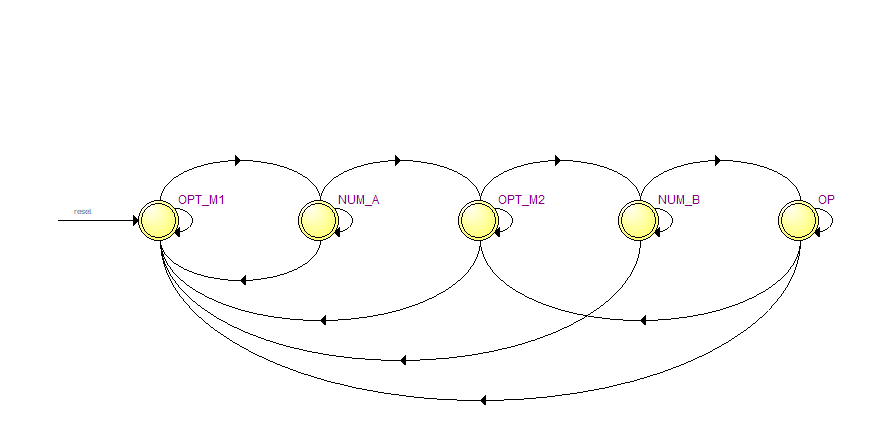
\includegraphics[width=\linewidth]
      {calculator_actual_state.pdf}
    \caption{Máquina de estados da calculadora.}
  \end{figure}

  Ao fim, a calculadora exibirá o resultado que, caso a pessoa
  entre com um próximo operador, pode ser utilizado para
  o próximo cálculo. Por exemplo, se quisermos calcular
  $5 \times -3$ e multiplicar por $-2$ o resultado, faríamos:

  \begin{table}[!htb]
    \centering
    \begin{tabular}{rm{3cm}}
      \keys{5} \keys{\mtp} \keys{\minus} \keys{3} \keys{\enter}
      & \includegraphics[scale=0.2]{7seg_-15.pdf} \\
      \keys{\mtp} \keys{\minus} \keys{2} \keys{\enter}
      & \includegraphics[scale=0.2]{7seg_30.pdf}
    \end{tabular}
  \end{table}

  A entrada de dados para a calculadora é feita exclusivamente
  pelo teclado numérico, onde as seguintes funções são definidas:

  \pagebreak

  \begin{table}[!htb]
    \centering
    \begin{tabular}{lll}
      \toprule
      \multicolumn{2}{l}{Função} & Teclas \\
      \midrule
      \multicolumn{2}{l}{\textit{Calculadora}} \\
      & Sinal de menos (para o número) & \keys{\minus} \\
      & Entrada de números & \keys{0} até \keys{9} \\
      & Multiplicação & \keys{\mtp} \\
      & Soma & \keys{\plus} \\
      & Subtração & \keys{\minus} \\
      & Calcular & \keys{\enter} \\
      & Reset & \keys{Backspace} \\
      \multicolumn{2}{l}{\textit{Controle de brilho}} \\
      & Diminuir o brilho & \keys{F1} \\
      & Aumentar o brilho & \keys{F2} \\
      \bottomrule
    \end{tabular}
    \caption{Funções da calculadora.}
  \end{table}

  Note que o controle de brilho é feito através de um módulo
  PWM, onde o controle do \emph{duty cicle} é exponencial.
  Como o valor inicial do brilho é $255_{(10)}$, pode-se
  demorar vários segundos para o brilho ter uma redução significativa.

  Os quatro \emph{displays} de sete segmentos (\texttt{HEX3} ao
  \texttt{HEX0}) são responsáveis por exibir a entrada digitada e
  saída do cálculo. O \emph{display} mais a esquerda representa 
  somente o sinal de menos do número, enquanto os outros três
  representam o número. Note que, por ser uma calculadora de
  \SI{8}{\bits} que opera em complemento de dois, as entradas
  permitidas são entre $-128$ e $127$. Caso ocorra algum 
  \emph{overflow} durante as operações, o LED vermelho mais a
  esquerda (\texttt{LEDR[9]}), localizado abaixo dos \emph{displays}
  se acenderá ao cálculo.

  A calculadora opera com uma máquina de estados, portanto é
  possível observar o estado atual que ela se encontra
  através dos LEDs vermelhos \texttt{LEDR[4]} ao \texttt{LEDR[0]},
  onde o \texttt{0} representa o primeiro estado e \texttt{4}
  representa o último.

  \section{Organização do projeto}

  O projeto foi dividido ao máximo tal que cada arquivo contenha
  poucas responsabilidades, para aumentar a organização e entendimento
  dos códigos. O projeto foi dividido nos seguintes arquivos:

  \begin{itemize}
    \item
    \texttt{full\_adder.vhd}: representa um somador completo, ou seja,
    permite o \emph{carry in};

    \item
    \texttt{adder\_nbits.vhd}: representa um somador de $n$ bits, é 
    utilizado para a soma e subtração em complemento de dois;

    \item
    \texttt{multiplier\_nbits.vhd}: representa um multiplicador de
    $n$ bits, onde a saída possui $2n$ bits. É implementado utilizando
    o Algoritmo de Booth, permitindo a operação com números em complemento
    de dois;

    \item
    \texttt{calculator\_kernel.vhd}: representa o núcleo da calculadora,
    similar a uma Unidade Lógica Aritmética, onde escolhe-se
    a operação e a efetua nos números de entrada;

    \item
    \texttt{calculator\_package.vhd}: pacote com algumas constantes
    para a escolha da operação no núcleo da calculadora;

    \item
    \texttt{clock\_divider.vhd}: representa um divisor de \emph{clock}
    genérico, utilizado somente para o controle do \emph{duty cicle}
    do módulo PWM;

    \item
    \texttt{pwm\_module.vhd}: representa um módulo PWM, que é utilizado
    para controlar o brilho dos quatro \emph{displays} de sete segmentos;

    \item
    \texttt{binary\_to\_bcd.vhd}: representa um conversor de binário de
    \SI{8}{\bits} para BCD, utilizando o Algoritmo \emph{Double dabble};

    \item
    \texttt{decoder\_bcd\_7seg.vhd}: representa um conversor de BCD
    para um \emph{display} de sete segmentos de ânodo comum.

    \item
    \texttt{keyboard\_keys.vhd}: pacote com as constantes que representam
    as teclas que podem ser utilizadas na calculadora e uma função
    que converte, quando possível, a tecla numérica para o binário dela.

    \item
    \texttt{ps2\_iobase.vhd}: módulo responsável pela comunicação
    com o protocolo PS2, é utilizado pelo controlador do teclado;

    \item
    \texttt{kbdex\_ctrl.vhd}: módulo responsável pela interface de
    controle do teclado PS2;

    \item
    \texttt{calculator.vhd}: principal arquivo da calculadora,
    responsável pela máquina de estados que a controla e a interação
    externa de entrada e saída, unindo todos os módulos necessários
    e efetuando a comunicação entre eles;

    \item
    \texttt{DE1\_pin\_assignments.csv}: designação de todos
    os pinos da placa.
  \end{itemize}

  \section{Problemas identificados e não resolvidos}

  Os seguintes problemas foram identificados após os testes:

  \begin{itemize}
    \item
    O \emph{overflow} da multiplicação pode não ser identificado
    corretamente em alguns casos específicos onde o resultado
    de \SI{16}{\bits}, ao ser reduzido para \SI{8}{\bits},
    possui o sinal correto que o resultado deveria ter, no entanto
    não representa o número correto referente ao resultado da
    multiplicação, pois o resultado foi reduzido para \SI{8}{\bits}.

    \item
    A entrada de números permite a entrada de números entre
    $-128$ e $127$. No entanto, se forem digitados mais de 
    3 dígitos ou os 3 digítos entrados superarem os limites
    superiores ou inferiores, o registrador que armazena
    o número lido não conterá o número correto. Por exemplo,
    se for digitado $132$, o número ficará como $-124$. Isto
    se deve à forma com qual os dígitos são manipulados na
    entrada.

    \item
    Algumas vezes, após ter entrado mais de 3 dígitos ou uma
    entrada inválida fora dos limites, a calculadora para de
    reconhecer novas teclas numéricas pressionadas e fica
    travada, possibilitando apenas usar alguma operação ou
    resetá-la.
  \end{itemize}

  \section{Autoria dos códigos utilizados}

  \begin{itemize}
    \item
    \texttt{full\_adder.vhd}: código original desenvolvido durante as aulas;

    \item
    \texttt{adder\_nbits.vhd}: código original desenvolvido durante as aulas.
    A detecção de \emph{overflow} foi baseada em uma resposta
    por GabrielOshiro. Disponível no StackOverflow:
    \url{https://stackoverflow.com/questions/32805087/how-is-overflow-detected-in-twos-complement};

    \item
    \texttt{multiplier\_nbits.vhd}: código baseado
    no Algoritmo de Booth, desenvolvido originalmente por
    Andrew Donald Booth, em 1950. Adaptado de:
    \url{https://en.wikipedia.org/wiki/Booth\%27s_multiplication_algorithm};

    \item
    \texttt{calculator\_kernel.vhd}: código original;

    \item
    \texttt{calculator\_package.vhd}: código original;

    \item
    \texttt{clock\_divider.vhd}: código original desenvolvido durante as aulas;

    \item
    \texttt{pwm\_module.vhd}: código original desenvolvido durante as aulas;

    \item
    \texttt{binary\_to\_bcd.vhd}: código baseado no Algoritmo
    Double dabble e desenvolvido durante as aulas. Adaptado de:
    \url{https://en.wikipedia.org/wiki/Double_dabble};

    \item
    \texttt{decoder\_bcd\_7seg.vhd}: código original desenvolvido durante as aulas;

    \item
    \texttt{keyboard\_keys.vhd}: código original;

    \item
    \texttt{ps2\_iobase.vhd}: cópia do código de terceiros.
    Desenvolvido pelo grupo do Prof\@. Mario Lúcio Côrtes;

    \item
    \texttt{kbdex\_ctrl.vhd}: cópia do código de terceiros.
    Desenvolvido pelo grupo do Prof\@. Mario Lúcio Côrtes;

    \item
    \texttt{calculator.vhd}: código original. Multiplicação
    por 10 durante a leitura foi adaptada de uma pergunta
    feita por Jack Smith. Disponível no StackOverflow:
    \url{https://stackoverflow.com/questions/10757966/bitshifting-to-multiply-an-integer-by-10};

    \item
    \texttt{DE1\_pin\_assignments.csv}: cópia do código de terceiros.
    Desenvolvido pelo grupo do Prof\@. Mario Lúcio Côrtes;
  \end{itemize}

  \section{Códigos desenvolvidos}

  \inputminted[label=full\_adder.vhd]{vhdl}{../calculator/full_adder.vhd}
  \inputminted[label=adder\_nbits.vhd]{vhdl}{../calculator/adder_nbits.vhd}
  \inputminted[label=multiplier\_nbits.vhd]{vhdl}{../calculator/multiplier_nbits.vhd}
  \inputminted[label=calculator\_kernel.vhd]{vhdl}{../calculator/calculator_kernel.vhd}
  \inputminted[label=calculator\_package.vhd]{vhdl}{../calculator/calculator_package.vhd}
  \inputminted[label=clock\_divider.vhd]{vhdl}{../calculator/clock_divider.vhd}
  \inputminted[label=pwm\_module.vhd]{vhdl}{../calculator/pwm_module.vhd}
  \inputminted[label=binary\_to\_bcd.vhd]{vhdl}{../calculator/binary_to_bcd.vhd}
  \inputminted[label=decoder\_bcd\_7seg.vhd]{vhdl}{../calculator/decoder_bcd_7seg.vhd}
  \inputminted[label=keyboard\_keys.vhd]{vhdl}{../calculator/keyboard_keys.vhd}
  \inputminted[label=calculator.vhd]{vhdl}{../calculator/calculator.vhd}

\end{document}